\documentclass{article}
\usepackage[utf8]{inputenc}
\usepackage{amsmath}
\usepackage{graphicx}
\usepackage{hyperref}
\usepackage{tikz}
\usepackage[a4paper,margin=1in,footskip=0.25in]{geometry}

\title{\textbf{Hypothetical Interventions on Sleep Stage Composition and Cognition and Brain Health} \protect\\ Analyis Plan}
\author{Lachlan Cribb \hspace{0.25cm} Beaudan Brown \and \\Stephanie Yiallourou \hspace{0.25cm} Matthew Pas\'e}
\date{\today}
\setlength{\parskip}{0.75em}
\begin{document}

\maketitle

\section{Introduction}
Insufficient slow wave sleep (SWS) has been associated with increased risk of dementia \cite{himali_association_2023}. SWS is thought to be important for glymphatic clearance of amyloid-$\beta$ and tau, the two hallmark features of Alzheimer's disease dementia. Restoring SWS may therefore reflect a potential intervention target to reduce risk of dementia. Similarly, an excessive proportion of time spent in light sleep (N1) has been associated with cognitive decline in older people \cite{song_relationships_2015}. A difficulty in interpreting these results, however, is the compositional nature of behavioural states. That is, time spent in each stage/state (N1, N2, N3, REM and wake) represents a compositional component of a 24 hour day. Therefore, if there is an increase in SWS, for example, then this time must come at the expense of another state (N1, N2, REM or wake). It may well be that the effect of increasing time in SWS depends on which other state(s) that time comes at the expense of.

Most, if not all, previous studies have utilised traditional regression tools, focusing on sleep stages in isolation. These methods assume that stages/states are independent of the other and unconstrained in time, which they are not (if one time use state increases another has to decrease). Thus, it is important to consider the co-dependent nature of time spent in behavioural states to determine the true effects of each state on health outcomes. To do this, we can apply the compositional data analysis (CoDA) approach, which treats states as inter-related within a constrained time period. This allows for estimating the association of reallocating time from one behavior/state to another on health outcomes whilst adjusting for the remaining state/behaviors. Thus, using this approach we can determine the benefits of increasing SWS at the expense of REM, for example, on cognitive and brain health as well as estimate an ideal composition (i.e., the ideal time spent in each state) of behavioural states for each outcome.

\section{Aims}
\begin{enumerate}
    \item To investigate the effect of different hypothetical interventions on sleep stage composition (the time spent in each state; N1, N2, N3, or REM) on cognitive function and MRI volumetric outcomes, compared to no intervention (not changing the sleep stage composition).
    \item To find the "ideal" pattern of sleep stage composition with respect to cognitive function and MRI volumetric outcomes. I.e., the absolute quantities of time spent in each state which is associated with the best cognitive performance and MRI volumetric outcomes.
\end{enumerate}

\section{Methods}

\subsection{Observational data}

Data are obtained from the Framingham Offspring Study (FOS) and the Sleep Heart Health Study (SHHS). SHHS is a multi-centre prospective cohort study designed to examine the cardiovascular outcomes of sleep-disordered breathing in middle-aged and older adults. Participants were recruited from multiple parent cohorts, including FOS, the Atherosclerosis Risk in Communities (ARIC) cohort, and the Cardiovascular Health Study (CHS). For this study, we used SHHS data provided by participants from the FOS study.

For SHHS, a sample of participants who met the inclusion criteria (see below) was invited to participate in the baseline SHHS examination (SHHS-1), which included a polysomnogram. A total of 997 individuals from the FOS study were enrolled between 1995 and 1998. A second polysomnogram (SHHS-2) was performed between 2001 and 2003 in 638 SOF participants.

\subsubsection{Eligibility criteria}

The following are the eligibility criteria for participation in SHHS:

\begin{itemize}
    \item Aged 40 or older
    \item No history of treatment for sleep apnea
    \item no Tracheostomy
    \item No current home oxygen therapy
\end{itemize}

\noindent For this study, we will additionally require that participants have SHHS-1 and SHHS-2 polysomnography data available and apply the following exclusion criteria:

\begin{itemize}
    \item Dementia or other significant neurological disease prior to SHHS-2
    \item Mild cognitive impairment prior to SHHS-2
    \item Significant cardiovascular disease prior to SHHS-2
    \item At least 4 hours of sleep at SHHS-1 and SHHS-2
    \item Sleep stage composition at SHHS-1 and SHHS-2 within expected bounds*
\end{itemize}

*We define expected bounds as X, Y, and Z.

\subsection{Hypothetical interventions}

Our exposure variables of interest are the time spent in each state, represented by the quintet $A = (W, SWS, N1, N2, REM)$ at SHHS-2. We use SHHS-2, rather than SHHS-1, for our exposure variables because it allows us to statistically adjust for sleep stage composition at SHHS-1. This ensures that the SHHS-2 sleep composition is approximately an "incident" exposure, thereby reducing confounding and selection bias related to past sleep behaviours.

The reference composition (the comparator for the hypothetical interventions we consider) is the observed sleep stage composition $A$. We estimate the mean outcome under this composition, represented in potential outcomes notation by $E[Y^A]$. The hypothetical interventions we consider are isotemporal modifications of $A$. That is, starting from the observed composition $A$, we add a time shift $\delta$ to one sleep stage $a_j$ and subtract it from $a_{j'}$ (e.g., adding 5 minutes to REM and subtracting it from SWS). For a given substitution of interest, We define the time-shift intervention as $d(A)$ and the composition resulting from applying the substitution as $A^d$. 

We will estimate the mean outcome after applying a given intervention, $E[Y^{A^d}]$. For every pair of sleep stage variables, we will apply 4 equally-spaced time shifts up to a maximum of $\Delta$. For example, if the maximum shift for a given pair of sleep stages variables is 20 minutes, we would consider 5, 10, 15, and 20 minute shifts.

The value of $\Delta$, for a given pair of sleep stage variables, is dependent on the sample data. We choose the largest whole number (in minutes) that produces a density ratio (the ratio of the density of $A^d$ to $A$, conditional on confounders; see Statistical Analysis section below) below the threshold $\lambda$ for all participants in the dataset.

\subsection{Outcomes}
\begin{itemize}
    \item Overall cognition factor score
    \item Domain specific cognition factor scores
    \item MRI volumetric outcomes (total brain volume, grey matter volume, white matter volume, hippocampal volume, white matter hyperintensities)
\end{itemize}

\subsection{Follow-up}
Follow-up commences at the time of SHHS-2 (the time of exposure measurement). Follow-up ends at loss to follow-up, death, or outcome measurement. 

\subsection{Confounders}

The presumed structure of confounding is displayed in the directed acyclic graph in Figure \ref{fig:dag}. $A$ represents sleep stage composition at SHHS-2, which is the exposure. $L_0$ represents confounders measured before but proximally to SHHS-2 and includes age, sex, education, race, MMSE score, body mass index (BMI), waist circumference, physical activity (from the PAI), hypertension, CVD, diabetes, smoking status, APOE $\epsilon$ 4 positivity, medication (sedative, sleeping pill, antidepressant), apnea hypopnea index, MRI intracranial volume (for MRI outcomes only) and SHHS1 Sleep macro-architecture measures time in N1, N2, N3, REM, time awake, wake after sleep onset (WASO), sleep maintenance efficiency, and apnea hypopnea index. $L$ represents covariates variables measured at time $t$. $U$ is a vector of unmeasured variables (e.g., genetics) which is a common cause of sleep stage composition, covariates $L_t$, death $D$, and the outcome $Y$.

\begin{figure}[h]
    \centering
    \usetikzlibrary{positioning}
    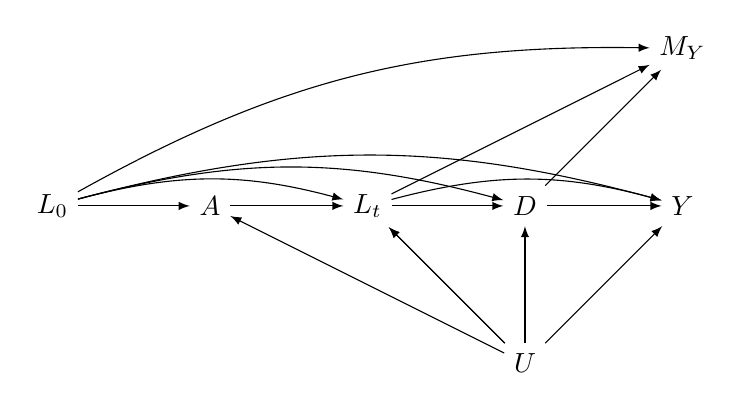
\begin{tikzpicture}[every node/.append style={draw, minimum size=0.5cm}]
        \node [draw=none] (L0) at (0,0) {$L_{0}$};
        \node [draw=none] (A) at (2,0) {$A$};
        \node [draw=none] (L) at (4,0) {$L_t$};
        \node [draw=none] (D) at (6,0) {$D$};
        \node [draw=none] (Y) at (8,0) {$Y$};
        \node [draw=none] (MY) at (8,2) {$M_Y$};
        \node [draw=none] (U) at (6,-2) {$U$};

        \draw [-latex] (L0) edge (A);
        \draw [-latex] (L0) edge [bend left=15] (L);
        \draw [-latex] (L0) edge [bend left=15](D);
        \draw [-latex] (L0) edge [bend left=15] (Y);
        \draw [-latex] (L0) edge [bend left=15] (MY);
        \draw [-latex] (L) edge (D);
        \draw [-latex] (L) edge [bend left=15] (Y);
        \draw [-latex] (L) edge (MY);
        \draw [-latex] (A) edge (L);
        \draw [-latex] (U) edge (D);
        \draw [-latex] (U) edge (A);
        \draw [-latex] (U) edge (Y);
        \draw [-latex] (U) edge (L);
        \draw [-latex] (U) edge (L);
        \draw [-latex] (D) edge (MY);
        \draw [-latex] (D) edge (Y);
    \end{tikzpicture}
    \caption{Directed acyclic graph}
    \label{fig:dag}
\end{figure}

\subsection{Statistical analysis}

\subsubsection{Isotemporal substitutions}

Before estimating treatment effects, we will transform compositional variables (time in N1, N2, N3, REM, WASO, and other wake) from the simplex to the unconstrained Real space using an isometric log-ratio transformation (ILR). These ILR coordinates will be used in subsequent steps.

To estimate the effect of increasing or decreasing time in a given sleep state, with that time coming at the expense of another state (e.g., an increase in SWS at the expense of REM) we will use the algorithm described in broad summary below:

\begin{itemize}
    \item Estimate $\Delta$, the largest substitution duration (in whole minutes) that results in a density ratio above the threshold $\lambda$
    \item Define a set of four equally spaced substitution durations, denoted by $\delta_1$, $\delta_2$, $\delta_3$, and $\delta_4$, where each $\delta_i$ is a whole number in minutes and $\delta_4$ = $\Delta$. 
    \item Estimate the mean outcome under no intervention $E[Y^C]$
    \item Estimate the mean outcome after applying the substitution of $d_i$ minutes, $E[Y^{A^d}]$, for all $i$ in 1 to 4
    \item Calculate the mean difference $E[Y^{A^d}]$ - $E[Y^A]$, representing the mean difference 
\end{itemize}

\subsubsection{Ideal and worst composition}

To estimate the ideal and worst composition, i.e., the absolute time spent in each sleep stage associated with the best and worst outcome, respectively, we will use the following method:

\section{References}
\bibliographystyle{plain}
\bibliography{citations}

\end{document}
